% !TeX document-id = {b4799037-fa3f-4e65-894b-ed263757f0b2}
% !TeX program = xelatex
% !BIB program = biber
% 独立编译的参考文献与补充材料，不计入主文档 8 页。
\documentclass[UTF8,a4paper,zihao=-4,fontset=fandol]{ctexart}
\newcommand{\DocumentType}{参考文献与补充材料}
% 共享排版设置。主文档与补充材料均使用 XeLaTeX。
\usepackage[a4paper,left=23mm,right=23mm,top=22mm,bottom=24mm]{geometry}
\usepackage{amsmath,amssymb,bm}
\usepackage{graphicx}
\usepackage{booktabs,tabularx,array}
\usepackage{enumitem}
\usepackage{xcolor}
\usepackage{caption,subcaption}
\usepackage{listings}
\usepackage{longtable}
\usepackage{makecell}
\usepackage{fancyhdr}
\usepackage[backend=biber,style=numeric,sorting=nyt]{biblatex}
\addbibresource{references.bib}
\usepackage[hidelinks,unicode]{hyperref}

\definecolor{hintgray}{RGB}{115,115,115}
\definecolor{rulegray}{RGB}{210,210,210}
\linespread{1.18}
\setlength{\parindent}{2em}
\setlength{\parskip}{0.15em}
\setlength{\emergencystretch}{2em}
\setlist{nosep,leftmargin=2em,topsep=0.3em}
\renewcommand{\arraystretch}{1.25}
\newcolumntype{Y}{>{\raggedright\arraybackslash}X}
\captionsetup{font=small,labelfont=bf,labelsep=quad}
\ctexset{
  section={format=\large\bfseries,beforeskip=1.2em,afterskip=0.6em},
  subsection={format=\normalsize\bfseries,beforeskip=0.9em,afterskip=0.4em},
  subsubsection={format=\normalsize\bfseries,beforeskip=0.5em,afterskip=0.2em}
}
\pagestyle{fancy}
\fancyhf{}
\fancyhead[L]{\small 安全强化学习方法复现报告}
\fancyhead[R]{\small \DocumentType}
\fancyfoot[C]{\small\thepage}
\setlength{\headheight}{15pt}
\renewcommand{\headrulewidth}{0.3pt}
\lstset{language=Python,basicstyle=\small\ttfamily,
  columns=fullflexible,keepspaces=true,breaklines=true,
  showstringspaces=false,frame=single,rulecolor=\color{rulegray},
  numbers=left,numberstyle=\tiny\color{hintgray},numbersep=8pt}

% 填写后删除相应占位命令。false 仅隐藏提示，不代表内容已经完成。
\newif\ifshowplaceholders
\showplaceholderstrue
\newcommand{\pending}{\ifshowplaceholders\textcolor{hintgray}{待补充}\fi}
\newcommand{\blankcontent}[1][1.2cm]{%
  \par\noindent\ifshowplaceholders{\color{hintgray}\small〔待补充〕}\par\fi
  \vspace{#1}}
\newcommand{\summaryitem}[1]{\par\noindent\textbf{#1}\quad\pending\par\vspace{0.5em}}
% 已填写的概述段落：\summarypara{小标题}{正文}
\newcommand{\summarypara}[2]{\par\noindent\textbf{#1}\quad #2\par\vspace{0.35em}}
% 行内代码/路径：可在 . / _ 处断行
\newcommand{\code}[1]{\nolinkurl{#1}}
\AtBeginDocument{\def\UrlBreaks{\do\.\do\/\do\_\do\-\do\=}}
% 含空格的命令行（\code 会吞掉空格）
\newcommand{\cmd}[1]{\texttt{\detokenize{#1}}}
\newcommand{\reporttitle}[1]{%
  \begin{center}
  {\LARGE\bfseries #1\par}\vspace{0.7em}
  {\normalsize 作者：范金鹏\qquad 日期：2026 年 11 月 8 日\par}
  \end{center}\vspace{0.5em}}


\usepackage{placeins}
\usepackage{needspace}
\usepackage{float}
\raggedbottom
\clubpenalty=10000
\widowpenalty=10000
\displaywidowpenalty=10000
\setlength{\textfloatsep}{11pt plus 2pt minus 2pt}
\setlength{\intextsep}{9pt plus 2pt minus 2pt}
\setlength{\floatsep}{10pt plus 2pt minus 2pt}
\setlength{\abovedisplayskip}{8pt plus 2pt minus 2pt}
\setlength{\belowdisplayskip}{8pt plus 2pt minus 2pt}
\setlength{\LTpre}{7pt}
\setlength{\LTpost}{9pt}
\captionsetup{skip=6pt}
\captionsetup[table]{position=top}
\renewcommand{\arraystretch}{1.18}
\renewcommand{\topfraction}{0.92}
\renewcommand{\bottomfraction}{0.85}
\renewcommand{\textfraction}{0.08}
\renewcommand{\floatpagefraction}{0.9}
\setcounter{topnumber}{3}
\setcounter{bottomnumber}{2}
\setcounter{totalnumber}{4}
\makeatletter
\setlength{\@fptop}{0pt}
\setlength{\@fpsep}{12pt}
\setlength{\@fpbot}{0pt plus 1fil}
\makeatother
\ctexset{
 section={beforeskip=0.95em,afterskip=0.45em},
 subsection={beforeskip=0.7em,afterskip=0.3em},
 subsubsection={beforeskip=0.55em,afterskip=0.25em},
 paragraph={beforeskip=0.65em,afterskip=0.55em}
}
\newcolumntype{P}[1]{>{\raggedright\arraybackslash}p{#1}}
\renewcommand{\thepage}{S\arabic{page}}
\begin{document}
\nocite{*}
\reporttitle{安全强化学习方法复现报告\\[0.3em]
  \large 参考文献与补充材料}

\printbibliography[heading=bibintoc,title={参考文献}]

\appendix
\ctexset{section={name={附录\space,},number=\Alph{section}}}
\numberwithin{equation}{section}
\numberwithin{figure}{section}
\numberwithin{table}{section}

\section{理论与模型补充推导}
\label{app:theory}
本附录补充正文第 2 节的模型推导与求解方法：先说明倒立摆残差的输入相关性、复合核 GP 后验及安全约束，再说明车辆跟随的位置积分与车距屏障。

\subsection{倒立摆}
\label{app:theory-pend}

沿用正文记号，$s=(\theta,\dot\theta)^\top$，$f(s)$、$g(s)$ 分别为名义漂移项和输入增益，$u$ 为执行力矩，$a=u^{CBF}$ 为安全修正。真实质量、杆长记为 $m,l$，名义值记为 $m_n,l_n$；重力加速度用 $g_0=10\,\mathrm{m/s^2}$ 表示，以区别输入增益 $g(s)$。令 $c=(\Delta t^2,\Delta t)^\top$，Pendulum-v0 的离散动力学（论文式 (17)）可写为
\begin{equation}
s_{t+1}=s_t+\begin{pmatrix}\dot\theta_t\,\Delta t\\0\end{pmatrix}
+\frac{3g_0}{2l}\sin\theta_t\,c+\frac{3}{ml^2}u_t\,c.
\label{eq:true}
\end{equation}
名义模型采用同一形式，将 $m,l$ 替换为 $m_n,l_n$，因此 $g(s)=\tfrac{3}{m_nl_n^2}c$。仿真器的角速度限幅为 $\pm60\,\mathrm{rad/s}$；以下推导针对未触发该限幅的转移。

\subsubsection{残差的输入相关性}
GP 的训练标签为实际下一状态与名义预测之差：
\begin{equation}
y_t=s_{t+1}-f(s_t)-g(s_t)u_t=d_f(s_t)+d_g(s_t)u_t.
\end{equation}
由式 \eqref{eq:true} 与名义模型相减，得到
\[
\begin{aligned}
d_f(s)&=\Bigl(\frac{3g_0}{2l}-\frac{3g_0}{2l_n}\Bigr)\sin\theta\,c,\\
d_g(s)&=\Bigl(\frac{3}{ml^2}-\frac{3}{m_nl_n^2}\Bigr)c.
\end{aligned}
\]
取 $m=l=1$、$m_n=l_n=1.4$，漂移误差的系数约为 $15-10.714=4.286$，输入增益误差的系数约为 $3-1.093=1.907$。因此，同一状态下的残差仍随力矩 $u$ 改变。只以状态为输入的 GP 无法区分这种差异，会将不同动作对应的残差混合拟合；CBF 改变候选动作时，原预测均值及方差也未显式反映残差随动作的变化。这正是采用复合核 GP 的原因。

\subsubsection{复合核 GP 的后验}
先对单个状态分量推导，暂省分量下标 $j$。设漂移误差与增益误差的先验独立，$d_f\sim\mathcal{GP}(0,k_f)$、$d_g\sim\mathcal{GP}(0,k_g)$，观测为
$y_t=d_f(s_t)+d_g(s_t)u_t+\nu_t$，其中 $\nu_t\sim\mathcal N(0,\sigma_\nu^2)$ 且相互独立。复合核\cite{umlauft2020feedback}给出
\begin{equation}
\operatorname{Cov}(y_t,y_\tau)=k_f(s_t,s_\tau)+u_t\,k_g(s_t,s_\tau)\,u_\tau+\sigma_\nu^2\delta_{t\tau},
\end{equation}
其中 $\delta_{t\tau}$ 为 Kronecker 符号。对 $N$ 条训练样本，记 $\mathsf S=[s_1,\ldots,s_N]^\top$、$Y=(y_1,\ldots,y_N)^\top$、$U=\operatorname{diag}(u_1,\ldots,u_N)$，则
$K=K_f+UK_gU+\sigma_\nu^2I$，其中 $(K_f)_{t\tau}=k_f(s_t,s_\tau)$，$K_g$ 同理。

在查询状态 $s_*$ 处，令 $w_*=(d_f(s_*),d_g(s_*))^\top$，其与 $Y$ 的互协方差为 $A^\top$，其中
\begin{equation}
A=\bigl[\,k_f(\mathsf S,s_*),\ U\,k_g(\mathsf S,s_*)\,\bigr]\in\mathbb R^{N\times2}.
\end{equation}
记两项先验标准差为 $\sigma_f,\sigma_g$。由高斯条件分布\cite{rasmussen2006gp}，后验均值和协方差为
\begin{equation}
\begin{aligned}
\mathbb E[w_*\mid Y]&=A^\top K^{-1}Y,\\
\Sigma_*&=\operatorname{diag}(\sigma_f^2,\sigma_g^2)-A^\top K^{-1}A.
\end{aligned}
\end{equation}
恢复分量下标，令 $z=(1,u)^\top$，则候选输入 $u$ 对应的残差预测为
\[
\mu_{d,j}(s_*,u)=\mu_{f,j}(s_*)+\mu_{g,j}(s_*)u,\qquad
\sigma_{d,j}(s_*,u)=\sqrt{z^\top\Sigma_{*,j}z}.
\]
将各分量组合，即得正文中的 $\mu_d(s,u)$ 与 $\sigma_d(s,u)$。实现中不显式计算 $K^{-1}$，而用 Cholesky 分解 $K=LL^\top$ 和 $V=L^{-1}A$ 计算后验协方差 $\Sigma_*=\operatorname{diag}(\sigma_f^2,\sigma_g^2)-V^\top V$，对应 \code{dynamics_gp.py} 的 \code{CompoundGP.predict}。

\paragraph{固定超参数。}
两个状态分量分别建立 GP。按 $(\theta,\dot\theta)$ 的顺序，先验标准差取
\[
\begin{aligned}
(\sigma_{f,1},\sigma_{f,2})^\top
 &=0.3\,\frac{3g_0}{2l_n}c
 \approx(8.04\times10^{-3},\,0.161)^\top,\\
(\sigma_{g,1},\sigma_{g,2})^\top
 &=0.5\,g(s)
 \approx(1.37\times10^{-3},\,2.73\times10^{-2})^\top.
\end{aligned}
\]
观测噪声标准差为 $\sigma_{\nu,j}=0.02\sigma_{f,j}$。平方指数核 $k_f,k_g$ 对 $(\theta,\dot\theta)$ 的长度尺度分别为 $(1,50)$、$(10,50)$。在 $k_\delta=1.5$ 下，先验输入增益的逐分量下置信界为 $g_j-k_\delta\sigma_{g,j}=0.25g_j>0$，保留了输入增益的符号。

\subsubsection{二阶锥约束与字典序求解}
固定当前状态 $s$，对仿射屏障 $h_i(s)=p_i^\top s+q_i$，记
\[
b_i=(1-\eta)h_i(s)-p_i^\top[f(s)+\mu_f(s)]-q_i,\qquad
\beta_i=p_i^\top[g(s)+\mu_g(s)].
\]
正文的安全约束可改写为
\begin{equation}
\phi_i(u)=b_i-\beta_iu+k_\delta\sum_j|p_{ij}|\,
\bigl\|\Sigma_j^{1/2}(1,u)^\top\bigr\|_2\le\epsilon,
\end{equation}
其中 $\Sigma_j$ 为当前状态处 $(d_{f,j},d_{g,j})$ 的后验协方差，$\Sigma_j^{1/2}$ 为其对称半正定平方根。每个 $\phi_i$ 均为凸函数，故 $\phi(u)=\max_i\phi_i(u)$ 也为凸函数，非空的可行集为闭区间。

令候选输入 $u_c=u^{RL}+\bar u_\phi$，力矩区间为 $\mathcal U=[-15,15]$。目标 $|u-u_c|+K_\epsilon\epsilon$ 在 $K_\epsilon\to\infty$ 时按字典序求解：
\[
\epsilon^*=\max\Bigl\{0,\min_{u\in\mathcal U}\phi(u)\Bigr\},\qquad
u^*=\underset{u\in\mathcal U,\,\phi(u)\le\epsilon^*}{\arg\min}\,|u-u_c|.
\]
也就是先最小化松弛量，再将候选输入投影到相应可行区间。程序用黄金分割法求 $\min\phi$，用二分法求区间端点，各迭代 100 次；随后检查力矩限幅、松弛量非负性，以及放宽后的约束余量是否不小于 $-10^{-7}$，检查失败即报错。$K_\epsilon=10^{12}$ 只用于记录目标值，不参与上述两步求解。

\subsubsection{作者代码问题的定量说明}
\paragraph{状态与动作错位。}
作者 DDPG-CBF 先更新状态再记录，日志中的状态、动作因此为 $S_i=s_{i+1}$、$U_i=u_i$。用于 GP 的标签为 $S_{i+1}-f(S_i)-g(S_i)U_i$。代入真实转移，得到
\begin{equation}
y_i^{\mathrm{old}}=d(s_{i+1},u_{i+1})+g(s_{i+1})(u_{i+1}-u_i).
\end{equation}
除真实残差外，标签还混入了相邻动作之差。策略变化与 OU 探索噪声都会影响这一项，却被 GP 当作模型误差学习。每回合还缺少第一条转移 $s_0\to s_1$，仅得到 199 条样本。

\paragraph{安全过滤后重新采样。}
设策略均值为 $\mu$，作者代码对 $\mu+\bar u_\phi$ 求得修正 $a$，过滤后第 $i$ 个约束的余量为 $M_i\ge0$。实际执行时又采样噪声 $\xi\sim\mathcal N(0,\sigma_\pi^2)$，得到 $u=\mu+\bar u_\phi+a+\xi$。在作者采用的状态 GP 模型下，余量随之变为
\[
M_i+p_i^\top g(s)\xi.
\]
当 $p_i^\top g(s)\xi<-M_i$ 时，采样动作会违反该约束。若 $M_i=0$ 且 $p_i^\top g(s)\ne0$，其概率为 $1/2$。此外，旧策略概率使用过滤后的均值，新策略概率却使用原始均值 $\mu'$。以新旧方差相同的情形为例，概率比为
\[
r=\frac{\mathcal N(u;\mu',\sigma_\pi^2)}{\mathcal N(u;\mu+\bar u_\phi+a,\sigma_\pi^2)}.
\]
即使新旧策略参数相同，$\mu'=\mu$，仍有 $r=\exp\{-[(u-\mu)^2-\xi^2]/(2\sigma_\pi^2)\}$，通常不等于 1。修改后使用原始策略样本及其分布参数计算概率比。

\paragraph{训练与预测的名义模型不一致。}
作者 TRPO-CBF 用 $m=l=2$ 计算训练标签，此时漂移和输入增益的系数分别为 7.5、0.375，标签为 $y=7.5\sin\theta\,c+2.625u\,c$。预测时却用真实参数 $m=l=1$，名义重力项已为 $15\sin\theta\,c$。因此，即使 GP 准确拟合了标签中的漂移误差，叠加后该项也会变为 $22.5\sin\theta\,c$；标签中的输入相关部分还会被额外计入。修改后训练与预测统一用名义值 1.4。

\subsection{车辆跟随}
\label{app:theory-car}
沿用正文 2.1.2 节的位置、速度记号；相邻车辆的位置差和速度差均按前车减后车定义。
\paragraph{位置积分错误引入的输入增益偏差。}
以第 4 辆车为例，记实际加速度为 $a_4=u-k_dv_4$（作者环境未对该车加噪声）。源码先更新速度，再用新速度积分位置，得到
\[
v_4^+=v_4+a_4\Delta t,\qquad
p_4^+=p_4+v_4^+\Delta t+\tfrac12a_4\Delta t^2
     =p_4+v_4\Delta t+\tfrac32a_4\Delta t^2.
\]
因此，源码仿真器中 $\partial p_4^+/\partial u=\tfrac32\Delta t^2$，而名义模型中的对应项为 $\tfrac12\Delta t^2$，相差 3 倍。当 $\Delta t=0.05\,\mathrm{s}$、$u=100\,\mathrm{m/s^2}$ 时，仅这一项就使单步位置预测相差 0.25\,m。该残差与输入成正比，无法用仅依赖状态的模型完整表示。

\paragraph{相对速度屏障与车距约束。}
记车距裕量 $e=\Delta p-2$，则 $\dot e=\Delta v$，正文构造的屏障为 $h=\dot e+\alpha e$。在连续时间下，若始终保持 $h\ge0$，则
\[
\frac{\mathrm d}{\mathrm dt}\bigl[\exp(\alpha t)e(t)\bigr]
=\exp(\alpha t)h(t)\ge0,
\qquad e(t)\ge e(0)\exp(-\alpha t).
\]
因此，从 $e(0)\ge0$ 的初态出发，保持 $h\ge0$ 即可维持 2\,m 车距约束。离散实现仍采用正文的条件 $h(s_{t+1})\ge(1-\eta)h(s_t)$。在修正后的位置积分下，输入对下一步屏障的作用为
\[
\frac{\partial h(s_{t+1})}{\partial u_t}
=\pm\Bigl(\Delta t+\frac{\alpha}{2}\Delta t^2\Bigr)
=\pm0.0525\,\mathrm{s}.
\]
其中正、负号分别对应车 4–5、车 3–4。满幅输入可使单步 $h$ 改变约 5.25\,m/s；纯车距屏障的相应变化仅为 0.125\,m。关键差别在于，引入相对速度后，控制输入通过 $\Delta t$ 的一阶项进入离散约束，而不再仅通过 $\Delta t^2$ 的位置项起作用。

\FloatBarrier
\section{代码修改说明}
\label{app:code}
本附录区分模型与任务调整、实现错误修正和训练配置调整。B.1、B.2 节分别给出倒立摆与车辆跟随的逐文件对照；表中行号对应本次实验使用的源码版本。

\subsection{倒立摆}
\label{app:code-pend}
作者源码位于 \code{RL-CBF-master/pendulum/}。修改后代码以每次运行保存的 \code{source/} 快照为准，例如 \code{pendulum/results/final_600ep/<ALG>/seed1/source/}；文件的 SHA256 见对应运行目录的 \code{run_config.json}。\code{learner.py} 与 \code{replay_buffer.py} 未修改。表 \ref{tab:codediff} 列出具体修改，关键问题的推导见附录 A.1.4。

{\small
\setlength{\extrarowheight}{2.5pt}
\begin{longtable}{@{}>{\raggedright\arraybackslash}p{27mm}>{\raggedright\arraybackslash}p{63mm}>{\raggedright\arraybackslash}p{64mm}@{}}
\caption{倒立摆实现与设置的修改对照}\label{tab:codediff}\\
\toprule
问题 & 作者源码 & 修改后 \\ \midrule
\endfirsthead
\caption[]{倒立摆实现与设置的修改对照（续）}\\
\toprule
问题 & 作者源码 & 修改后 \\ \midrule
\endhead
\midrule
\multicolumn{3}{r@{}}{\footnotesize 续下页}\\
\endfoot
\endlastfoot
\multicolumn{3}{@{}l}{\textbf{模型与安全约束调整（正文 2.1.1 节）}}\\*
残差模型 & \code{dynamics_gp.py}：sklearn GP，输入 $s$；DDPG-CBF 核为 \code{1.0*RBF(2)+White(0.1)}，TRPO-CBF 为 \code{C*RBF(10)}；通过最大似然估计选择超参数，优化重启 10 次 & \code{dynamics_gp.py:24-47} 复合核 \code{CompoundGP}，超参数固定；\code{:114-117} 计算 $\sigma_{d,j}(s,u)$ \\
CBF 约束形式 & \code{cbf.py}：cvxopt 二次规划，$\sigma$ 与 $u$ 无关 & \code{cbf.py:47-95}：二阶锥约束，按字典序求解 \\
安全集 & DDPG-CBF \code{cbf.py:20-24}：$\pm\theta\pm0.05\dot\theta$；TRPO-CBF 中角速度项系数为 0.01 & \code{cbf.py:17-18}：\code{H=[[1,0],[-1,0]]} \\
目标与松弛 & \code{P=diag(1,1e24)}（DDPG-CBF）或 \code{diag(1,1e16)}（TRPO-CBF）；$\epsilon$ 无非负约束 & 先最小化非负松弛量，再最小化修正幅值 $|a|$ \\
速度约束 & 硬约束；DDPG-CBF 中候选动作被计入两次（\code{cbf.py:44-45}） & 默认关闭，可用 \code{--enforce-speed-limit} 开启，开启时只计入一次 \\
\multicolumn{3}{@{}l}{\textbf{代码错误修正（正文 2.2 节）}}\\*
转移错位 & DDPG-CBF \code{ddpg.py:364-371} 先执行 \code{s=s2} 再记录 & \code{ddpg.py:291,308-310} 分别保存 \code{Observation}、\code{Action}、\code{NextObservation} \\
Actor 动作范围 & DDPG-CBF \code{ddpg.py:411,417}：\code{env.action_space.high} 实测为 2 & \code{ddpg.py:371}：同步包装器的动作空间，范围为 $\pm15$ \\
先过滤后采样 & TRPO-CBF \code{trpo.py:280-292} & \code{trpo.py:288-295}：先采样，再补偿、过滤 \\
概率比 & \code{trpo.py:289,298}：旧策略均值含 $\bar u_\phi+a$ & \code{trpo.py:162,310-311}：使用 \code{Action_RL} 及原始分布参数 \\
名义模型 & TRPO-CBF \code{dynamics_gp.py:29-30} 用 $m=l=2$，\code{:63-64} 用 $m=l=1$ & \code{dynamics_gp.py:10,66-75}：训练与预测统一用名义值 1.4 \\
时间截断 & DDPG \code{ddpg.py:296-299}、DDPG-CBF \code{:326-329} 存为终止；TRPO \code{gae.py:54,72-74} 令 $V(s_T)=0$ & DDPG \code{env_done} 排除截断；TRPO \code{gae.py:97-112} 用 $V(s_T)$ 自举 \\
GAE 跨回合 & \code{gae.py:80} 在整批序列上计算 & \code{gae.py:103-109} 逐条轨迹计算 \\
KL 检查 & \code{utils.py:162-177} 只检查代理目标是否下降 & \code{utils.py:174-204} \code{TRUST_REGION_STEP}：实际 KL 超过上限时回退 \\
GP 更新时机 & DDPG-CBF \code{ddpg.py:280-284,387-388}；TRPO-CBF \code{trpo.py:246-250,322-323}：每批只拟合前 4 个回合，滞后一轮使用 & 每个回合后重新拟合，并在下一个回合使用 \\
补偿网络 & DDPG-CBF \code{ddpg.py:390-394} 仅训练 $i\le4$，使用累计路径；TRPO-CBF 在策略更新前用均值修正训练 & 每 5 个回合用最近一批训练，标签与 $s_t$ 对齐，首轮输出为零 \\
\multicolumn{3}{@{}l}{\textbf{训练配置调整}}\\*
价值网络 & \code{gae.py:103-108} 每次一步约束共轭梯度 & \code{gae.py:171-181}：Adam，10 个 epoch，批量 64，学习率 $10^{-3}$，回报标准化 \\
\multicolumn{3}{@{}l}{\textbf{次要问题}}\\*
鲁棒项 & TRPO-CBF \code{cbf.py:35}：$k_\delta|p^\top\sigma|$ & $k_\delta|p|^\top\sigma$。对该屏障，两者相同 \\
角度残差 & 未对 $\pm\pi$ 做周期处理 & \code{dynamics_gp.py:89} 将角度残差折回 $[-\pi,\pi)$ \\
事后裁剪 & DDPG-CBF \code{cbf.py:59-64} 在求解后改写修正量 & 将力矩限幅纳入求解区间，约束检查失败时报错 \\
存储动作 & DDPG \code{ddpg.py:294,298} 存未裁剪动作 & 先裁剪到动作范围再存储 \\
\bottomrule
\end{longtable}
}

\paragraph{训练配置调整。}
为使四种算法在相同条件下比较，统一环境与初态（\code{fair_environment.py}），并采用表 \ref{tab:params} 的训练参数。观测缩放与归一化由 \code{obs_norm.py} 处理；DDPG 改用高斯探索噪声，TRPO 初始标准差设为 3。倒立摆原实现的 BN 层处于推理模式，滑动统计量未更新，相当于固定归一化后的可学习仿射变换；修改后为统一网络配置而移除。这里的 BN 调整与车辆算例中单样本训练模式下的 BN 错误不同。

\paragraph{DDPG-CBF：转移记录与动作范围。}
作者代码先更新状态，再记录用于 GP 和补偿网络的数据：
\begin{lstlisting}
s = s2
obs.append(s); action.append(action_)
\end{lstlisting}
这使状态与动作错位一步，修改后显式保存 $(s_t,u_t,s_{t+1})$。此外，作者只修改内层 \code{env.unwrapped.action_space}，外层 \code{env.action_space} 在 Gym 0.17.3 中仍为 $[-2,2]$，Actor 因而仍限幅于 $\pm2$。保持非零摆角静止需要 $|u|=5|\sin\theta|$；在考察的 $|\theta|\le1$ 区间内，Actor 无法独自平衡 $|\theta|>\arcsin(2/5)\approx0.41$ 的状态。修改后同步内外层动作空间为 $\pm15$。

\paragraph{TRPO-CBF：采样与策略更新。}
作者在过滤后的均值周围重新采样：
\begin{lstlisting}
u_bar_ = cbf.control_barrier(self, np.squeeze(prev_obs_expanded),
                           action_dist_mu_RL, f, g, x, std)
action_dist_mu_ = action_dist_mu_RL + u_bar_
action_ = np.random.normal(loc=action_dist_mu_,
                          scale=np.exp(action_dist_logstd_))
\end{lstlisting}
修改后先从原始策略采样，再补偿并过滤，执行前不再添加采样噪声；策略更新使用原始样本及其分布参数。时间截断时采用价值自举，GAE 按回合计算，线搜索拒绝实际 KL 超限的更新。沿用原线搜索的中间版本短测中，实际 KL 曾达到 0.98。GP 原先滞后 5–9 回合更新，DDPG-CBF 的补偿网络则在第 25 回合后冻结；修改后分别按回合更新 GP、按迭代更新补偿网络。

\subsection{车辆跟随}
\label{app:code-car}
作者源码位于 \code{RL-CBF-master/car/<ALG>/}，修改后代码位于仓库 \code{car/}。TRPO 与 TRPO-CBF 共用 \code{TRPO-CBF/} 的实现；DDPG 与 DDPG-CBF 共用 \code{DDPG-CBF/ddpg.py}，并从 \code{TRPO-CBF/} 导入仿真器等模块。两条基线通过 \code{--no_cbf} 关闭安全滤波及补偿。表 \ref{tab:carcodediff} 的“修改后”栏中，未另注目录的文件均位于 \code{TRPO-CBF/}；源码 SHA256 保存在各运行的 \code{run_config.json} 中。

{\small
\setlength{\extrarowheight}{2.5pt}
\begin{longtable}{@{}>{\raggedright\arraybackslash}p{25mm}>{\raggedright\arraybackslash}p{64mm}>{\raggedright\arraybackslash}p{65mm}@{}}
\caption{车辆跟随实现与设置的修改对照}\label{tab:carcodediff}\\
\toprule
问题 & 作者源码 & 修改后 \\ \midrule
\endfirsthead
\caption[]{车辆跟随实现与设置的修改对照（续）}\\
\toprule
问题 & 作者源码 & 修改后 \\ \midrule
\endhead
\midrule
\multicolumn{3}{r@{}}{\footnotesize 续下页}\\
\endfoot
\endlastfoot
\multicolumn{3}{@{}l}{\textbf{任务设置、模型与安全约束调整（正文 2.1.2 节）}}\\*
制动规则 & 四份 \code{car_simulator.py:51-52,62-63}：车距 $<6$ 时 \code{action - k_brake*gap}（车 5 针对车 3，阈值 12\,m、系数减半），名义模型采用同一规则 & \code{car_simulator.py:25-27}：$-k_b\max(0,6-\Delta p)$，名义模型共用 \code{driver_controls} \\
软惩罚阈值 & \code{car_simulator.py:105-109}：$d<2.99$，$|500/d|$ & \code{car_simulator.py:49-50}：$d\le3$，下限 0.5\,m \\
燃油项 & DDPG \code{car_simulator.py:94} 用 $|v_4|$，其余用 $v_4$ & 四种算法统一使用 $v_4$ \\
屏障 & TRPO-CBF \code{cbf.py:19-27}：8 行 $\Delta p\pm0.001v-2$；DDPG-CBF \code{cbf.py:20-28} 系数 0.002 & \code{cbf.py:19-24}：2 行 $\Delta v+2(\Delta p-2)$ \\
QP 求解 & \code{cbf.py:17,57}：cvxopt，\code{P=diag(1,1e18)}（DDPG-CBF 1e20），松弛量不返回；\code{:60-65} 事后截断并打印 “Error in QP” & \code{cbf.py:35-66}：闭式解，返回松弛量 \\
GP 模型 & \code{dynamics_gp.py:18-21}：sklearn \code{C*RBF}，\code{alpha=0.5}，10 次重启，15 维绝对状态输入 & \code{dynamics_gp.py:20-28,68-72}：固定超参数，6 维相对特征；\code{:104} 方差计入观测噪声 \\
GP 标定 & 无 & \code{trpo.py:221-249}：训练前 400 步随机输入（独立环境），不计入训练量 \\
\multicolumn{3}{@{}l}{\textbf{代码错误修正（正文 2.2 节）}}\\*
位置积分 & 四份 \code{car_simulator.py:32-33}：先更新速度，再用新速度积分 & \code{car_simulator.py:110-111}：使用更新前的速度积分位置 \\
回放池视图 & DDPG \code{car_simulator.py:83-89,205}、\code{ddpg.py:291}；DDPG-CBF \code{ddpg.py:332}：存入同一数组的视图 & \code{car_simulator.py:95-96} 返回副本；DDPG-CBF \code{ddpg.py:63-67,152,176} 复制到预分配数组 \\
BN 训练模式 & DDPG \code{ddpg.py:75,78,162,268}；DDPG-CBF \code{ddpg.py:274}：\code{tflearn.is_training(True)}，单样本调用 & DDPG-CBF \code{ddpg.py:93-104}：移除 BN \\
补偿网络 & TRPO-CBF \code{trpo.py:134-138,272-273}：只在前 9 次迭代训练，从一开始使用；DDPG-CBF \code{ddpg.py:308-313}：补偿输出固定为零，\code{:391-392} 用全部累计路径训练 & \code{trpo.py:138-142,181-182}、DDPG-CBF \code{ddpg.py:157-158,209-212}：首轮为 0，每次迭代用最近一批训练并使用 \\
先过滤后采样 & TRPO-CBF \code{trpo.py:269-289}：对均值求 CBF，再重新采样 & \code{trpo.py:176-190}：先采样，再补偿、过滤 \\
GP 更新 & TRPO-CBF \code{trpo.py:247-251,327-328}、DDPG-CBF \code{ddpg.py:281-285,388-389}：每批只用一个回合（79 点），滞后一批使用 & \code{dynamics_gp.py:79-94}：每个回合后用最近 200 条转移重新拟合 \\
TRPO 观测错位 & TRPO \code{trpo.py:228,248,264}：观测序列为 $(s_0,s_0,s_1,\dots,s_{78})$ & \code{trpo.py:175,200-206}：显式保存 \code{NextObservation} \\
终止标志 & TRPO \code{car_simulator.py:68}：\code{L=100} 而回合为 80 步，\code{reset} 不清零计数 & \code{car_simulator.py:67}：每回合清零，长度统一由 \code{config.py} 给出 \\
GAE 与截断 & \code{gae.py:72-80}：在整批序列上计算，时间截断视为终止 & \code{gae.py:58-73}：逐条轨迹计算，截断时用 $V(s_T)$ 自举 \\
KL 检查 & \code{trpo.py:160-178}、\code{utils.py:166-181}：只检查代理目标 & \code{utils.py:144-173}：实际 KL 超限即拒绝 \\
名义模型 & \code{car_simulator.py:158-193}：读取仿真器当前车辆对象，而非传入的状态 & \code{car_simulator.py:31-46}：改为仅依赖传入状态的函数；原先误读的分量不进入 CBF 或 GP，未影响本次结果 \\
\multicolumn{3}{@{}l}{\textbf{次要问题}}\\*
策略标准差 & \code{trpo.py:52} 按自身行数平铺，只影响记录的熵 & 按批量大小平铺 \\
领头车 & $a_1=k_p(v_{\mathrm{des}}(t)-v_1)$，与论文式 (27) 字面 $a_1=v_{\mathrm{des}}-10\sin0.2t$ 不同 & 未修改 \\
\bottomrule
\end{longtable}
}

\paragraph{训练配置与记录。}
完整设置见表 \ref{tab:carparams} 和附录 E.2。奖励在学习更新时乘以 0.01，报告仍使用未缩放回报；TRPO 的采样动作在计算概率比前截断到 $\pm100$。DDPG 每 5 回合记录并更新一次补偿网络，初态与环境噪声使用独立随机数流。以上调整与表中的实现错误修正分别记录。

每回合的 \code{episodes.csv} 记录回报、修正量及补偿量 RMS、松弛量和实际 CBF 条件违反次数，并同步生成 TensorBoard 日志。模型每 25 次迭代保存一次；中文路径通过 ASCII 目录链接兼容原运行环境。

\FloatBarrier
\section{补充实验结果}
\label{app:experiments}
本附录给出逐种子结果及约束诊断。回报指回合累计奖励；“前 100”“末 100”均为对应回合的平均回报。碰撞和越界按回合计数，同一回合发生多次仅计一次。修正量与补偿量先逐回合计算 RMS，再对指定回合区间取平均。

\subsection{倒立摆}
\label{app:exp-pend}
\subsubsection{修改后代码的训练结果}
图 \ref{fig:safetycbf}、\ref{fig:perseed} 补充正文的越界、修正量及逐种子回报曲线，表 \ref{tab:perseed} 给出数值结果。数据由 \code{figures/make_pendulum_figs.py} 计算，完整数值见 \code{figures/pendulum_metrics.json}。
\begin{figure}[H]
\centering
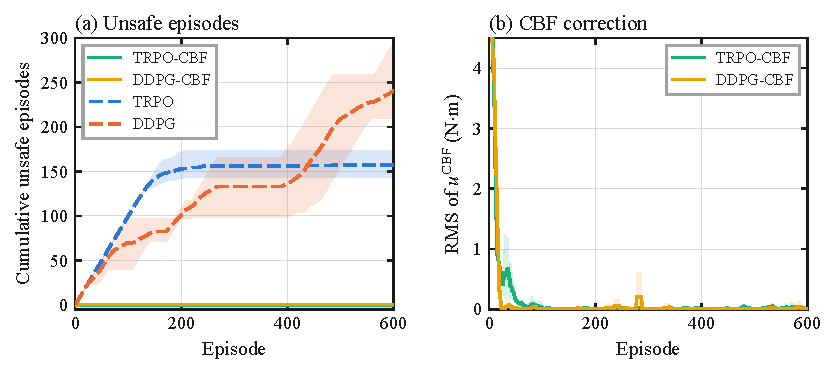
\includegraphics[width=0.95\linewidth]{figures/pendulum_safety_cbf.pdf}
\caption{倒立摆的累计越界与 CBF 修正量（修改后代码，种子 1–3）。(a) 累计越界回合数；(b) 每回合修正量 $u^{CBF}$ 的 RMS，作 10 回合滑动平均。粗线为三个种子的均值，阴影为最小值到最大值的范围。}
\label{fig:safetycbf}
\end{figure}




{\small\setlength{\tabcolsep}{4pt}
\begin{longtable}{@{}llrrcrl@{}}
\caption{倒立摆各随机种子的训练指标（修改后代码，各 600 回合）}\label{tab:perseed}\\
\toprule
算法 & 种子 & \makecell{前 100\\回报} & \makecell{后 100\\回报} & \makecell{越界数\\1–100 / 101–300 / 301–600} & \makecell{最大摆角\\（rad）} & \makecell{松弛量 $>0$\\的回合} \\ \midrule
\endfirsthead
\caption[]{倒立摆各随机种子的训练指标（续）}\\
\toprule
算法 & 种子 & \makecell{前 100\\回报} & \makecell{后 100\\回报} & \makecell{越界数\\1–100 / 101–300 / 301–600} & \makecell{最大摆角\\（rad）} & \makecell{松弛量 $>0$\\的回合} \\ \midrule
\endhead
\midrule
\multicolumn{3}{r@{}}{\footnotesize 续下页}\\
\endfoot
\endlastfoot
TRPO & 1 & $-1678$ & $-3.39$ & 100 / 73 / 1 & 3.142 & — \\
TRPO & 2 & $-1284$ & $-3.26$ & 100 / 53 / 2 & 3.142 & — \\
TRPO & 3 & $-1040$ & $-3.32$ & 100 / 43 / 0 & 3.142 & — \\
DDPG & 1 & $-630$  & $-65.4$  & 40 / 95 / 82   & 3.141 & — \\
DDPG & 2 & $-1765$ & $-173.6$ & 97 / 1 / 111   & 3.141 & — \\
DDPG & 3 & $-3159$ & $-108.4$ & 71 / 95 / 129  & 3.142 & — \\
TRPO-CBF & 1 & $-144.8$ & $-3.10$ & 0 / 0 / 0 & 0.99996 & 1 \\
TRPO-CBF & 2 & $-103.6$ & $-4.27$ & 0 / 0 / 0 & 0.99996 & 1, 4 \\
TRPO-CBF & 3 & $-117.5$ & $-3.19$ & 0 / 0 / 0 & 0.99996 & 1 \\
DDPG-CBF & 1 & $-28.0$ & $-3.57$ & 0 / 0 / 0 & 0.99997 & 1, 7, 8 \\
DDPG-CBF & 2 & $-27.6$ & $-3.33$ & 0 / 0 / 0 & 0.99997 & 1, 5, 7, 9 \\
DDPG-CBF & 3 & $-33.5$ & $-5.60$ & 1 / 0 / 0 & 1.103 & 1, 7, 8 \\
\bottomrule
\end{longtable}
}

\paragraph{安全性与训练波动。}
两种 CBF 版本首回合回报约为 $-150$ 至 $-200$。TRPO 基线前 100 回合均越界，第 300 回合后基本不再越界；DDPG 的越界持续至训练结束。TRPO-CBF 种子 2 与 DDPG-CBF 种子 3 在后期偶有较差回报（图 \ref{fig:perseed}）。正松弛仅出现在前 9 回合，最大值为 0.096，对应 DDPG-CBF 种子 3 的第 7 回合，也是唯一一次越界。

\begin{figure}[H]
\centering
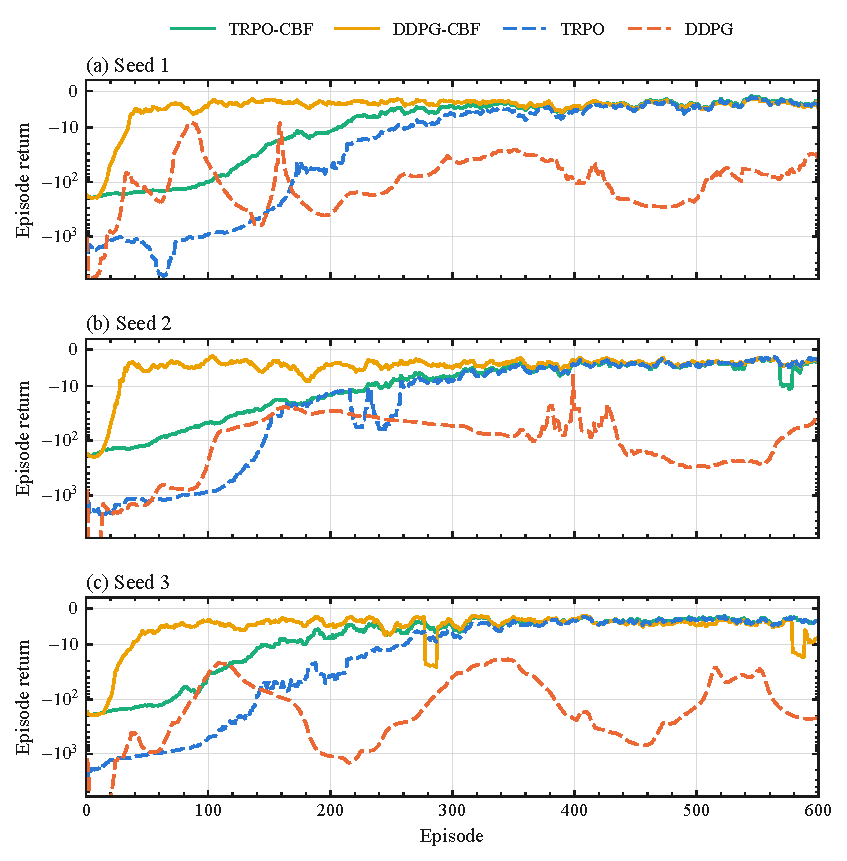
\includegraphics[width=0.9\linewidth]{figures/pendulum_return_per_seed.pdf}
\caption{倒立摆各随机种子的训练回报（修改后代码，各 600 回合）。每个子图对应一个种子，四种算法共用初态序列。曲线为 10 回合滑动平均，纵轴采用对称对数刻度（$|R|\le10$ 的部分为线性）。正文图 1(b) 汇总这三组曲线的均值与范围。}
\label{fig:perseed}
\end{figure}

\subsubsection{作者源码在默认设置下的结果}
图 \ref{fig:original}、表 \ref{tab:orig} 给出源码原样重跑的结果。作者文件与默认超参数均保留，仅由外部脚本补设种子并关闭 \code{env.render()}。默认训练长度为：DDPG 600 回合，DDPG-CBF 150 轮、每轮 5 回合，共 750 回合；TRPO 和 TRPO-CBF 各 9015 回合。后两者的停止条件为步数严格大于 $1.8\times10^6$，因而多运行一批。图中比较前 600 回合，表中另列完整训练结束时的回报。

\paragraph{统计口径与任务差异。}
逐回合数据由 \code{figures/extract_original.py} 从作者输出的 \code{.mat} 提取。DDPG 类记录执行后状态，TRPO 类记录执行前状态，最大摆角均取每回合 200 个记录状态的最大值。CBF 版本从安全集内出发，记录时点差异不改变其越界计数。作者两条基线使用 $\pm2$ 力矩，初始摆角 $\theta_0\sim U[-\pi,\pi]$，任务与 CBF 版本不同，其越界数主要反映初态分布和摆起过程。

\paragraph{主要现象。}
TRPO-CBF 种子 1、2 在第 64–65 回合达标，种子 3 在前 600 回合未达标，三个阶段的越界数为 6、97、229。种子 3 的最大摆角仅 1.007\,rad，与策略停留在边界附近、过滤后重新采样引起小幅越界的现象相吻合。DDPG-CBF 最大摆角约 1.34\,rad，末 100 回合回报为 $-63$ 至 $-96$，修正量 RMS 由初期种子均值 7.7 降至各种子的 1.8–4.4\,N·m，训练后仍依赖安全滤波。



\begin{figure}[H]
\centering
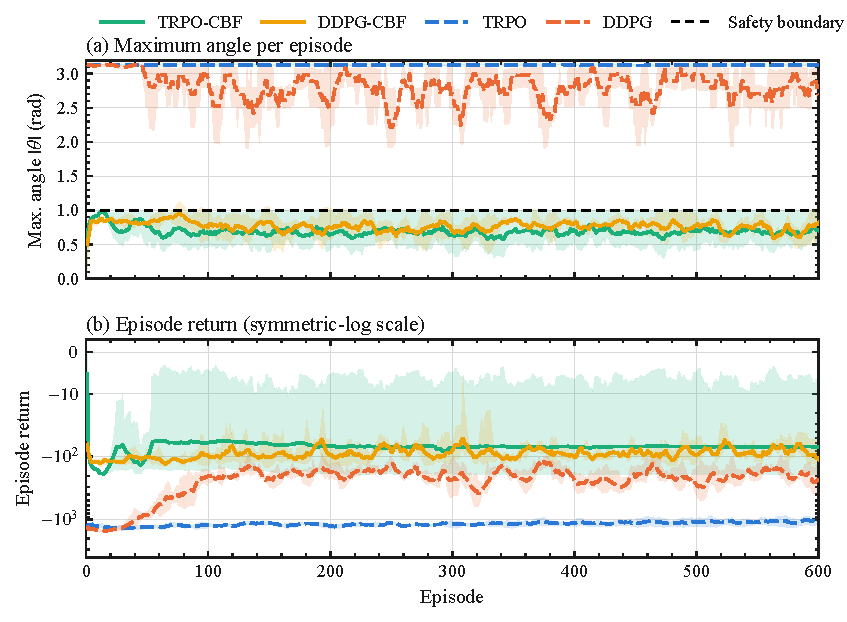
\includegraphics[width=0.9\linewidth]{figures/pendulum_original_training.pdf}
\caption{倒立摆作者源码的训练曲线（默认设置，种子 1–3，前 600 回合）。平滑及种子汇总方式同正文图 1。两条基线使用 $\pm2$ 力矩，$\theta_0\in[-\pi,\pi]$，任务设置与 CBF 版本不同，相关指标不宜直接比较。TRPO-CBF 的均值主要受未收敛的种子 3 影响，种子 1、2 的回报接近阴影上沿。}
\label{fig:original}
\end{figure}

{\small\setlength{\tabcolsep}{2.5pt}
\begin{longtable}{@{}llrrcrrr@{}}
\caption{作者源码各随机种子指标（默认设置）}\label{tab:orig}\\
\toprule
算法 & 种子 & \makecell{前 100\\回报} & \makecell{第 501–600\\回报} & \makecell{前 600 个的越界数\\1–100 / 101–300 / 301–600} & \makecell{最大摆角\\（rad）} & \makecell{完整训练\\回合数} & \makecell{完整训练末\\100 个回报} \\ \midrule
\endfirsthead
\caption[]{作者源码各随机种子指标（续）}\\
\toprule
算法 & 种子 & \makecell{前 100\\回报} & \makecell{第 501–600\\回报} & \makecell{前 600 个的越界数\\1–100 / 101–300 / 301–600} & \makecell{最大摆角\\（rad）} & \makecell{完整训练\\回合数} & \makecell{完整训练末\\100 个回报} \\ \midrule
\endhead
\midrule
\multicolumn{3}{r@{}}{\footnotesize 续下页}\\
\endfoot
\endlastfoot
TRPO$^\dagger$ & 1 & $-1280$ & $-972.3$  & 100 / 200 / 300 & 3.142 & 9015 & $-901.4$ \\
TRPO$^\dagger$ & 2 & $-1248$ & $-1017.3$ & 100 / 200 / 300 & 3.142 & 9015 & $-167.2$ \\
TRPO$^\dagger$ & 3 & $-1345$ & $-1246.7$ & 100 / 200 / 300 & 3.142 & 9015 & $-469.8$ \\
DDPG$^\dagger$ & 1 & $-718$  & $-221.5$ & 95 / 173 / 266  & 3.142 & 600 & $-221.5$ \\
DDPG$^\dagger$ & 2 & $-784$  & $-166.5$ & 94 / 179 / 272  & 3.142 & 600 & $-166.5$ \\
DDPG$^\dagger$ & 3 & $-902$  & $-212.9$ & 98 / 175 / 273  & 3.142 & 600 & $-212.9$ \\
TRPO-CBF & 1 & $-57$  & $-8.2$   & 1 / 0 / 0     & 1.002 & 9015 & $-8.2$ \\
TRPO-CBF & 2 & $-44$  & $-7.1$   & 9 / 0 / 0     & 1.007 & 9015 & $-5.4$ \\
TRPO-CBF & 3 & $-162$ & $-194.0$ & 6 / 97 / 229  & 1.007 & 9015 & $-38.2$ \\
DDPG-CBF & 1 & $-102$ & $-95.7$  & 12 / 46 / 69  & 1.344 & 750 & $-93.6$ \\
DDPG-CBF & 2 & $-122$ & $-88.4$  & 20 / 22 / 25  & 1.329 & 750 & $-93.2$ \\
DDPG-CBF & 3 & $-107$ & $-62.9$  & 13 / 5 / 19   & 1.288 & 750 & $-55.6$ \\
\bottomrule
\multicolumn{8}{@{}p{\linewidth}@{}}{$^\dagger$ 作者基线为 $\pm2$ 力矩、$\theta_0\in[-\pi,\pi]$ 的摆起任务。完整训练中 TRPO-CBF 种子 3 共越界 616 次。}
\end{longtable}
}




\FloatBarrier
\subsection{车辆跟随}
\label{app:exp-car}
图 \ref{fig:carorig}–\ref{fig:carperseed}、表 \ref{tab:carperseed} 给出车辆跟随的逐种子结果，数据由 \code{figures/make_car_figs.py} 计算，完整数值见 \code{figures/car_metrics.json}。

\paragraph{作者源码：安全性与训练后期表现。}
两种 CBF 版本均无碰撞，但存在小幅 2\,m 越界：TRPO-CBF 出现在种子 1 第 2068 回合和种子 3 第 29 回合，最小车距分别为 1.968、1.925\,m；DDPG-CBF 出现在种子 2 的第 149–358 回合之间，共 10 回合，最小车距为 1.93–1.98\,m。TRPO-CBF 种子 1 末 1000 回合中，仍有一半回合的修正量 RMS 大于 1\,m/s$^2$，种子 2、3 则均不超过该值。DDPG-CBF 全部 1000 回合的修正量平均 RMS 为 40–51\,m/s$^2$，每回合均有 CBF 介入；回报虽从约 $-4.8\times10^4$ 提高至 $-2.9\times10^4$，第 4 辆车仍贴近约 2.26\,m 行驶，修正量反而增大。

TRPO 三个种子在前 600 回合分别碰撞 310、452、599 次，最后一次碰撞发生在第 13556、10579、21316 回合，默认训练结束时均不再碰撞。DDPG 的车距中位数为 0.63、$-3.93$、$-13.53$\,m，回报最低约为 $-7.2\times10^7$；作者环境在两车穿过后继续仿真，$|500/d|$ 在 $d\to0$ 附近会产生很大的惩罚。

\paragraph{修改后：松弛量与模型置信区间。}
CBF 采用闭式解，未发生求解器数值失败，最大松弛量为 0.25。TRPO-CBF 仅种子 1 的第 6 回合、种子 2 的第 4 回合出现正松弛；DDPG-CBF 三个种子分别有 7、12、3 回合出现正松弛。其中种子 1 为第 1、10、546、551、556、559、606 回合，种子 2 分布在第 4–1295 回合，种子 3 为第 11、26、67 回合。

对整回合松弛量均为零的记录，统计实际转移不满足 $h(s_{t+1})\ge(1-\eta)h(s_t)$ 的回合数。模型预测可行而实际条件未满足，说明相应置信区间未覆盖该步残差。TRPO-CBF 三个种子分别有 1、5、2 个此类回合，均发生于前 64 回合；DDPG-CBF 分别有 87、102、209 个，分布于整个训练过程，这些回合均未越界。DDPG 的碰撞仅发生在前 8000 步；TRPO 种子 3 在 13.3 万步后不再碰撞。TRPO-CBF 种子 3 的末 100 回合回报与收敛后的 TRPO 相当（$-715$ 对 $-738$）。DDPG-CBF 末 100 回合的补偿输出 RMS 分别为 94.0、98.0、92.1\,m/s$^2$，种子 3 的 CBF 修正量仍为 10.3\,m/s$^2$。

\paragraph{作者日志的统计方式。}
\code{figures/extract_car_original.py} 将作者 \code{.mat} 按 80 步切分回合，TRPO 类每批 1200 步。TRPO、TRPO-CBF、DDPG-CBF 记录执行前状态；DDPG 因状态数组被原地改写而记录执行后状态，均已与固定初态核对。作者代码不返回 QP 松弛量，表中记为“未记录”。重跑时未出现 \texttt{Error in QP} 提示，但这不能代替松弛量统计。

\begin{figure}[H]
\centering
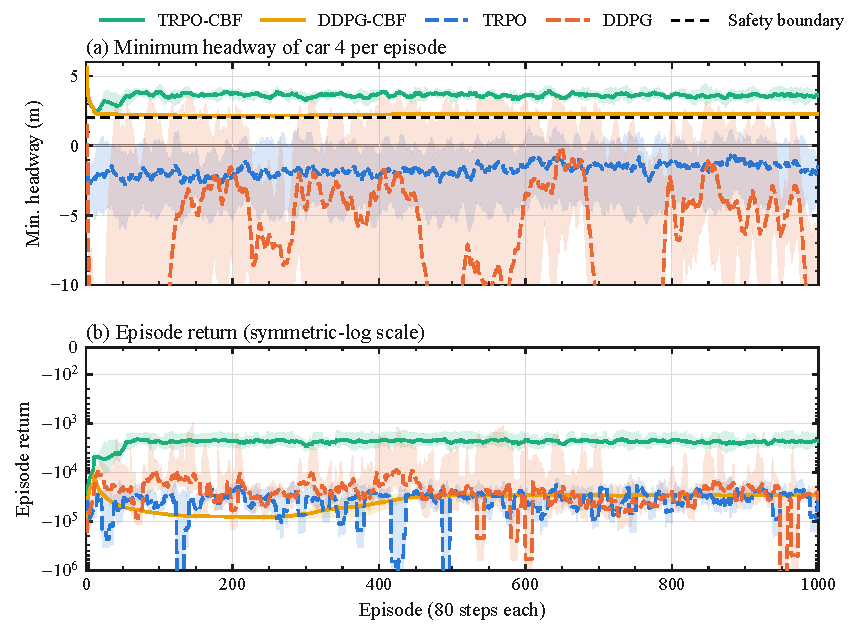
\includegraphics[width=0.9\linewidth]{figures/car_original_training.pdf}
\caption{车辆跟随作者源码的训练曲线（默认设置，种子 1–3，前 1000 回合）。每回合 80 步，横轴为回合；两种 DDPG 的全部训练均在图内，TRPO 类完整结果见表 \ref{tab:carperseed}。(a) 每回合最小车距，纵轴显示 $[-10,6]$\,m，DDPG 的实际最低值约为 $-153$\,m；(b) 回报，采用对称对数刻度。平滑及种子汇总方式同正文图 3。}
\label{fig:carorig}
\end{figure}

\begin{figure}[H]
\centering
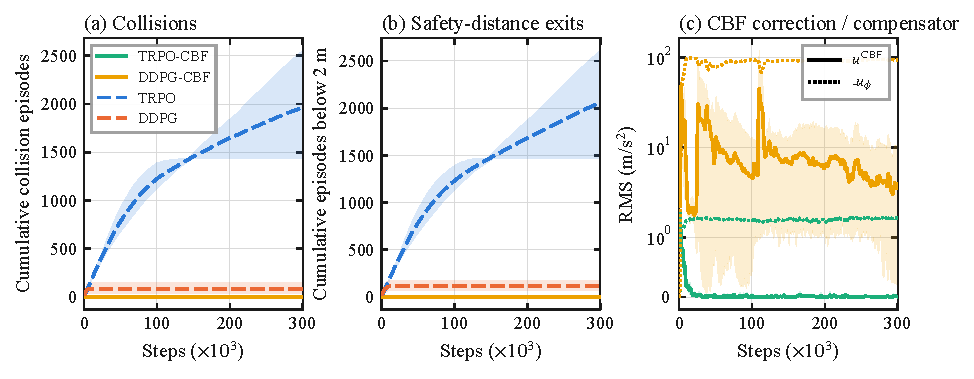
\includegraphics[width=\linewidth]{figures/car_safety_cbf.pdf}
\caption{车辆跟随的累计安全事件与安全修正（修改后代码，种子 1–3，横轴为环境步数）。(a) 累计碰撞回合数；(b) 累计 2\,m 越界回合数；(c) CBF 修正量 $u^{CBF}$ 的 RMS（实线）及补偿输出 $\bar u_\phi$ 的 RMS（点线），采用对称对数刻度。曲线经 10 回合滑动平均后取种子均值，阴影为最小值到最大值的范围。}
\label{fig:carsafety}
\end{figure}



\begin{figure}[H]
\centering
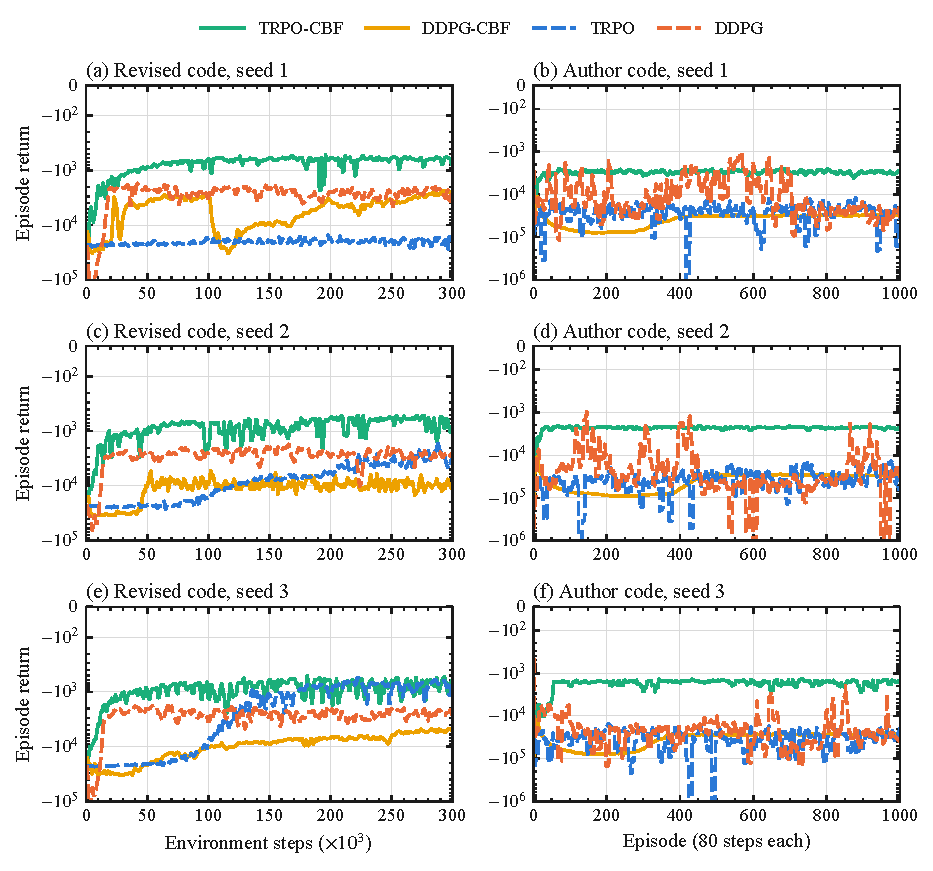
\includegraphics[width=\linewidth]{figures/car_per_seed.pdf}
\caption{车辆跟随各随机种子的训练回报。左列为修改后代码，横轴为环境步数；右列为作者源码的前 1000 回合，横轴为回合。曲线均作 10 回合滑动平均，纵轴采用对称对数刻度。修改后，同一子图内四种算法共用初态与噪声序列；作者 TRPO 类的种子由外部脚本设置。}
\label{fig:carperseed}
\end{figure}

{\footnotesize\setlength{\tabcolsep}{2.3pt}
\begin{longtable}{@{}llrrrcrrcc@{}}
\caption{车辆跟随各随机种子的训练指标}\label{tab:carperseed}\\
\toprule
算法 & 种子 & \makecell{回合\\数} & \makecell{前 100\\回报} & \makecell{末 100\\回报} & \makecell{碰撞回合数\\（训练回合四等分）} & \makecell{越界\\数} & \makecell{最小\\间距} & \makecell{修正量 RMS\\前 10 → 末 100} & \makecell{松弛量 $>0$\\的回合数} \\ \midrule
\endfirsthead
\caption[]{车辆跟随各随机种子的训练指标（续）}\\
\toprule
算法 & 种子 & \makecell{回合\\数} & \makecell{前 100\\回报} & \makecell{末 100\\回报} & \makecell{碰撞回合数\\（训练回合四等分）} & \makecell{越界\\数} & \makecell{最小\\间距} & \makecell{修正量 RMS\\前 10 → 末 100} & \makecell{松弛量 $>0$\\的回合数} \\ \midrule
\endhead
\midrule
\multicolumn{3}{r@{}}{\footnotesize 续下页}\\
\endfoot
\endlastfoot
\multicolumn{10}{@{}p{\linewidth}@{}}{\textit{作者源码，默认设置（每个回合 80 步）}}\\
TRPO & 1 & 22515 & $-59731$ & $-2617$ & 1234 / 10 / 3 / 0 & 3634 & $-6.82$ & — & — \\
TRPO & 2 & 22515 & $-73579$ & $-1734$ & 823 / 2 / 0 / 0 & 3575 & $-6.74$ & — & — \\
TRPO & 3 & 22515 & $-47948$ & $-2118$ & 5583 / 1484 / 14 / 12 & 9824 & $-10.82$ & — & — \\
DDPG & 1 & 1000 & $-23740$ & $-36413$ & 104 / 79 / 52 / 227 & 623 & $-66.77$ & — & — \\
DDPG & 2 & 1000 & $-33339$ & $-887181$ & 142 / 128 / 248 / 170 & 804 & $-70.97$ & — & — \\
DDPG & 3 & 1000 & $-20708$ & $-28026$ & 247 / 249 / 201 / 181 & 927 & $-152.63$ & — & — \\
TRPO-CBF & 1 & 15015 & $-3849$ & $-3496$ & 0 / 0 / 0 / 0 & 1 & 1.97 & 13.40 → 4.50 & 未记录 \\
TRPO-CBF & 2 & 15015 & $-2968$ & $-1981$ & 0 / 0 / 0 / 0 & 0 & 2.14 & 12.04 → 0.00 & 未记录 \\
TRPO-CBF & 3 & 15015 & $-4573$ & $-1438$ & 0 / 0 / 0 / 0 & 1 & 1.93 & 15.34 → 0.00 & 未记录 \\
DDPG-CBF & 1 & 1000 & $-47777$ & $-30741$ & 0 / 0 / 0 / 0 & 0 & 2.08 & 22.03 → 31.16 & 未记录 \\
DDPG-CBF & 2 & 1000 & $-49705$ & $-29802$ & 0 / 0 / 0 / 0 & 10 & 1.93 & 20.64 → 30.45 & 未记录 \\
DDPG-CBF & 3 & 1000 & $-47466$ & $-26267$ & 0 / 0 / 0 / 0 & 0 & 2.09 & 22.31 → 26.98 & 未记录 \\ \midrule
\multicolumn{10}{@{}p{\linewidth}@{}}{\textit{修改后代码（每个回合至多 200 步，$3\times10^5$ 步）}}\\
TRPO & 1 & 2652 & $-23645$ & $-19845$ & 660 / 640 / 627 / 637 & 2620 & $-0.25$ & — & — \\
TRPO & 2 & 2219 & $-23014$ & $-2928$ & 555 / 544 / 535 / 274 & 2099 & $-0.56$ & — & — \\
TRPO & 3 & 2395 & $-23068$ & $-738$ & 599 / 599 / 234 / 0 & 1471 & $-0.38$ & — & — \\
DDPG & 1 & 1550 & $-88097$ & $-2485$ & 69 / 0 / 0 / 0 & 100 & $-1.51$ & — & — \\
DDPG & 2 & 1625 & $-38224$ & $-2825$ & 151 / 0 / 0 / 0 & 177 & $-1.53$ & — & — \\
DDPG & 3 & 1525 & $-46149$ & $-2447$ & 35 / 0 / 0 / 0 & 69 & $-1.58$ & — & — \\
TRPO-CBF & 1 & 1500 & $-4957$ & $-631$ & 0 / 0 / 0 / 0 & 0 & 2.46 & 1.38 → 0.00 & 1 \\
TRPO-CBF & 2 & 1500 & $-5180$ & $-872$ & 0 / 0 / 0 / 0 & 0 & 2.48 & 1.46 → 0.01 & 1 \\
TRPO-CBF & 3 & 1500 & $-5573$ & $-715$ & 0 / 0 / 0 / 0 & 0 & 2.41 & 1.29 → 0.01 & 0 \\
DDPG-CBF & 1 & 1500 & $-24901$ & $-2556$ & 0 / 0 / 0 / 0 & 0 & 2.37 & 33.32 → 0.37 & 7 \\
DDPG-CBF & 2 & 1500 & $-32259$ & $-9926$ & 0 / 0 / 0 / 0 & 0 & 2.33 & 40.64 → 1.11 & 12 \\
DDPG-CBF & 3 & 1500 & $-27669$ & $-5085$ & 0 / 0 / 0 / 0 & 0 & 2.38 & 17.91 → 10.25 & 3 \\
\bottomrule
\multicolumn{10}{@{}p{\linewidth}@{}}{最小间距为全程最小值，单位 m；修正量 RMS 单位 m/s$^2$。作者环境在两车穿过后继续仿真，间距可为负。两组回报仅作组内比较。}
\end{longtable}
}



\paragraph{训练所得策略的闭环仿真。}
正文图 4 使用各次训练最后保存的策略，部署在修改后的真实动力学上。模型迭代次数见表 \ref{tab:carsim}：CBF 版本与 DDPG 通常为第 300 次，DDPG 种子 2 为第 325 次，TRPO 为第 250–275 次。执行采用确定性动作，CBF 版本保留补偿网络与安全滤波器；GP 重新标定，并用 5 个预热回合拟合后冻结。

所有算法与种子共用 \code{allCars(init_seed=2026, noise_seed=3026)} 生成的初态和噪声，仿真 200 步（10\,s）。车 1–3 不受第 4 辆车控制影响，因此各算法面对相同的前车，其速度由约 30 降至 20\,m/s。模型来自 \code{car/results/car_final/<ALG>/seed<k>/checkpoint/}；表 \ref{tab:carsim} 汇总三个种子的指标，图 \ref{fig:carsimseeds} 补充种子 2、3 的轨迹及 CBF 修正。回报按原奖励逐步累加，含 3\,m 软约束惩罚；此处未加入探索噪声，回报与训练时不宜直接比较。

{\footnotesize\setlength{\tabcolsep}{2.6pt}
\begin{longtable}{@{}llccccrcc@{}}
\caption{车辆跟随训练结束时策略的闭环仿真指标（修改后代码，10\,s）}\label{tab:carsim}\\
\toprule
算法 & 种子 & \makecell{模型\\迭代} & 碰撞 & \makecell{最小车距（m）\\及出现时刻} & \makecell{输入 RMS\\（m/s$^2$）} & 回报 & \makecell{$u^{CBF}$ RMS\\（m/s$^2$）} & \makecell{CBF 介入\\步数比例} \\ \midrule
\endfirsthead
\caption[]{车辆跟随训练结束时策略的闭环仿真指标（续）}\\
\toprule
算法 & 种子 & \makecell{模型\\迭代} & 碰撞 & \makecell{最小车距（m）\\及出现时刻} & \makecell{输入 RMS\\（m/s$^2$）} & 回报 & \makecell{$u^{CBF}$ RMS\\（m/s$^2$）} & \makecell{CBF 介入\\步数比例} \\ \midrule
\endhead
\midrule
\multicolumn{3}{r@{}}{\footnotesize 续下页}\\
\endfoot
\endlastfoot
TRPO-CBF & 1 & 300 & 否 & $3.31$ (8.6\,s) & $1.3$ & $-580$ & 0.00 & 0\% \\
TRPO-CBF & 2 & 300 & 否 & $3.60$ (8.2\,s) & $1.2$ & $-562$ & 0.00 & 0\% \\
TRPO-CBF & 3 & 300 & 否 & $3.63$ (8.1\,s) & $1.2$ & $-552$ & 0.00 & 0\% \\
DDPG-CBF & 1 & 300 & 否 & $3.21$ (8.0\,s) & $1.6$ & $-1024$ & 0.00 & 0\% \\
DDPG-CBF & 2 & 300 & 否 & $2.46$ (7.6\,s) & $1.6$ & $-22996$ & 1.40 & 62\% \\
DDPG-CBF & 3 & 300 & 否 & $2.83$ (8.6\,s) & $4.3$ & $-5943$ & 11.69 & 55\% \\
TRPO & 1 & 275 & 是（7.0\,s） & $-0.03$ (7.0\,s) & $0.7$ & $-15310$ & — & — \\
TRPO & 2 & 250 & 否 & $0.76$ (10.0\,s) & $2.7$ & $-2537$ & — & — \\
TRPO & 3 & 275 & 否 & $3.31$ (8.2\,s) & $1.3$ & $-627$ & — & — \\
DDPG & 1 & 300 & 否 & $3.10$ (5.2\,s) & $1.3$ & $-627$ & — & — \\
DDPG & 2 & 325 & 否 & $3.29$ (4.0\,s) & $1.8$ & $-792$ & — & — \\
DDPG & 3 & 300 & 否 & $3.08$ (5.2\,s) & $1.3$ & $-662$ & — & — \\
\bottomrule
\multicolumn{9}{@{}p{\linewidth}@{}}{“模型迭代”为最后保存的模型所对应的训练迭代次数；TRPO 因碰撞提前结束回合，$3\times10^5$ 步内未到第 300 次迭代。}
\end{longtable}
}
\begin{figure}[H]
\centering
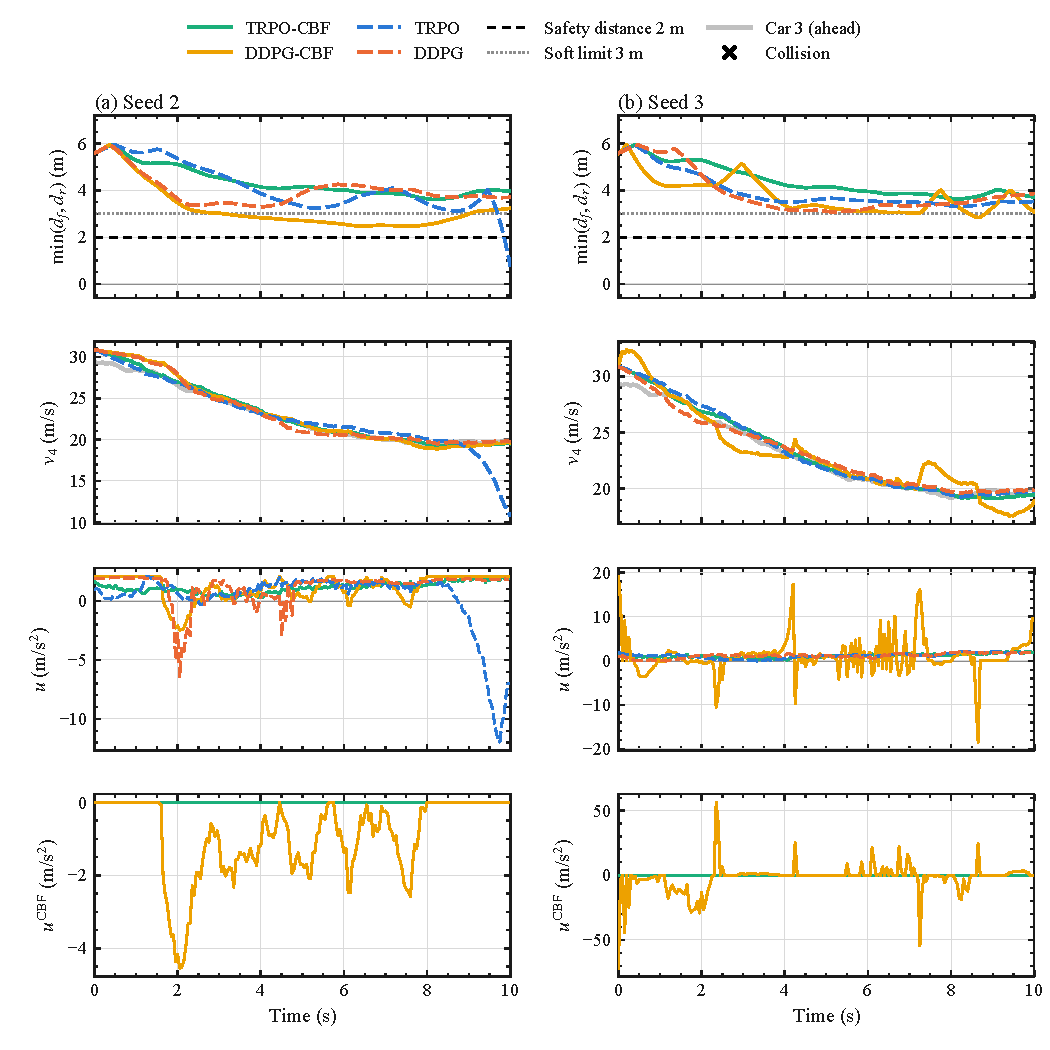
\includegraphics[width=0.95\linewidth]{figures/car_final_sim_seeds.pdf}
\caption{车辆跟随训练后策略的闭环响应（种子 2、3，设置同正文图 4）。自上而下为第 4 辆车与前、后车的最小间距、车速（灰线为车 3）、执行输入，以及两种 CBF 版本的修正量 $u^{CBF}$。DDPG-CBF 种子 3 的修正量在 $-72$ 至 $+56$\,m/s$^2$ 之间变化，至仿真末期仍有明显介入。}
\label{fig:carsimseeds}
\end{figure}

DDPG-CBF 种子 2 的回报远低于其他运行，其车距有 5.9\,s 处于 2–3\,m 之间，持续产生软约束惩罚，同时仍满足 2\,m 安全间距。完整数值见 \code{figures/car_final_sim.json}。

闭环仿真数据进一步显示，DDPG-CBF 种子 1 的 Actor、补偿网络与执行输入均值分别为 $-91.9$、$93.1$、$1.2$\,m/s$^2$；种子 2 分别为 $100.0$、$-97.9$、$1.2$\,m/s$^2$，其中 Actor 全程处于输出上限。种子 3 的 Actor 在 66\% 的步数上满足 $|u^{RL}|\ge95$，Actor、补偿网络与执行输入均值分别为 $-22.7$、$25.7$、$1.1$\,m/s$^2$。输出抵消的方向随种子变化。这些输出日志支持正文关于相互抵消偏置与饱和的机理分析；梯度减弱仍属于推断，最终版本未做消融或梯度测量。



\section{复现运行说明}
\label{app:reproduction}
两个算例均在 Windows 11、CPU 环境运行，使用 Python 3.7.9、TensorFlow 1.15.0、tflearn 0.3.2、Gym 0.17.3、NumPy 1.18.5、SciPy 1.4.1、scikit-learn 0.22.2.post1 和 cvxopt 1.2.7，绘图使用 matplotlib 3.2.2。代码、数据与 TensorBoard 日志位于仓库 \code{RL-CBF-Reproduction/}，目录结构见 \code{README.md}。以下按算例列出参数、训练命令和评估流程；命令中的目录参数需替换为实际路径。

\Needspace{6\baselineskip}
\subsection{倒立摆}
\label{app:repro-pend}
{\small
\begin{longtable}{@{}P{28mm}P{63mm}P{63mm}@{}}
\caption{倒立摆完整参数（修改后设置）}\label{tab:params}\\
\toprule
项目 & DDPG / DDPG-CBF & TRPO / TRPO-CBF \\ \midrule
\endfirsthead
\caption[]{倒立摆完整参数（续）}\\
\toprule
项目 & DDPG / DDPG-CBF & TRPO / TRPO-CBF \\ \midrule
\endhead
\midrule
\multicolumn{3}{r@{}}{\footnotesize 续下页}\\
\endfoot
\endlastfoot
环境 & \multicolumn{2}{P{\dimexpr126mm+2\tabcolsep\relax}@{}}{Pendulum-v0，$m=l=1$，$g_0=10$，$\Delta t=0.05$，力矩 $\pm15$，角速度 $\pm60$，每个回合 200 步；初态 $\theta_0,\dot\theta_0\sim U[-1,1]$，由 \code{RandomState(1234+seed)} 生成} \\
种子与训练量 & \multicolumn{2}{P{\dimexpr126mm+2\tabcolsep\relax}@{}}{种子 1、2、3；启动上限为 2000 回合，获得前 600 回合后停止并截取，报告这 600 回合的结果} \\
折扣与更新参数 & $\gamma=0.99$；目标网络软更新系数 $\tau=10^{-3}$ & $\gamma=0.99$，$\lambda=0.95$ \\
网络 & Actor、Critic 隐藏层均为 400–300 ReLU，无 BN；Actor 输出为 $15\tanh$ & 策略网络 64-64 ReLU；价值网络 100-50-25 tanh \\
优化 & Actor 学习率 $10^{-4}$，Critic 学习率 $5\times10^{-4}$，批量 256，回放池 $10^5$，每步更新 & KL $\le0.005$，回溯 20 次；价值网络用 Adam（$10^{-3}$，10 个 epoch，批量 64） \\
探索 & 独立高斯噪声 $\sigma=1$ & 初始 $\log\sigma=\ln3$ \\
观测处理 & 运行均值与方差归一化，截断到 $\pm10$，每 5 个回合更新 & 固定缩放 $[\cos\theta,\sin\theta,\dot\theta/8]$ \\
迭代 & 补偿网络与归一化每 5 个回合更新一次 & 每批 1000 步（5 个回合）\\
CBF & \multicolumn{2}{P{\dimexpr126mm+2\tabcolsep\relax}@{}}{$h=1\pm\theta$，$\eta=0.5$，$k_\delta=1.5$，$\epsilon\ge0$，按字典序求解；无速度约束；名义模型 $m=l=1.4$；复合核 GP 超参数见附录 A.1.2，每个回合后用该回合的 200 条转移重新拟合} \\
补偿网络 & \multicolumn{2}{P{\dimexpr126mm+2\tabcolsep\relax}@{}}{50-40 ReLU，最多 100 个梯度步，步长 10，线搜索回溯 30 次；输入与策略网络使用相同的观测处理} \\
\bottomrule
\end{longtable}
}

\Needspace{8\baselineskip}
\paragraph{训练与运行记录。}
以下路径均相对于仓库的 \code{pendulum/}。四种算法的训练入口分别位于 \code{DDPG/}、\code{DDPG-CBF/}、\code{TRPO/}、\code{TRPO-CBF/}。单次运行命令为
\begin{lstlisting}[language={},numbers=none,frame=none,breakatwhitespace=true,aboveskip=5pt,belowskip=7pt]
python scripts/run_one.py --alg TRPO-CBF --seed 1 --episodes 600 --run-dir <RUN_DIR>
\end{lstlisting}
脚本显式传入表 \ref{tab:params} 的超参数，将源码复制到运行目录的 \code{source/}，并在 \code{run_config.json} 中记录命令行参数和源码 SHA256。运行目录必须为新目录；每回合输出一行 \code{LIVE} 指标。\code{scripts/launch_all.py} 用于并行启动多个算法和种子，\code{scripts/export_first_n.py} 截取前 $N$ 回合，生成 \code{results/final_600ep/}。

\paragraph{训练前后策略的闭环评估。}
正文图 2 使用 \code{scripts/run_ckpt.py} 重跑种子 1，其训练配置与 \code{run_one.py} 相同，仅通过外部包装增加检查点保存。训练前后全部 TensorFlow 变量分别保存在 \code{ckpt/first}、\code{ckpt/last}，另存最终 GP 状态及 TRPO 参数。评估命令为
\begin{lstlisting}[language={},numbers=none,frame=none,breakatwhitespace=true,aboveskip=5pt,belowskip=7pt]
python scripts/eval_ckpt.py --run-dir <RUN_DIR>
\end{lstlisting}
脚本重建计算图并恢复策略参数，从 \code{RandomState(2026)} 生成的同一组 10 个初态出发，以确定性动作各仿真 200 步（10\,s）。初始策略配合零补偿与 GP 先验，训练后策略配合训练所得补偿网络与最终 GP 后验；两阶段均保留安全滤波，评估期间不更新 GP。轨迹写入 \code{eval_first_last.npz}，结果目录为 \code{results/checkpoint_rerun_seed1/}。

\paragraph{作者源码原样重跑。}
\begin{lstlisting}[language={},numbers=none,frame=none,breakatwhitespace=true,aboveskip=5pt,belowskip=7pt]
python scripts/launch_orig.py --root <RUN_ROOT> --orig-root <ORIG_ROOT>/pendulum
\end{lstlisting}
脚本原样复制作者文件，仅在外部补设种子并关闭渲染。作者输出的 \code{.mat} 共约 515\,MB，未纳入仓库；\code{results/author_code_default/} 保存从中提取的逐回合 \code{episodes.csv}、\code{run_config.json} 和控制台日志。提取脚本为 \code{report/figures/extract_original.py}。

\paragraph{图表与 TensorBoard。}
在 \code{report/} 下运行
\begin{lstlisting}[language={},numbers=none,frame=none,breakatwhitespace=true,aboveskip=5pt,belowskip=7pt]
python figures/make_pendulum_figs.py
\end{lstlisting}
脚本读取逐回合 CSV 与 \code{eval_first_last.npz}，生成倒立摆图形及 \code{pendulum_metrics.json}。在 \code{pendulum/} 下运行 \cmd{python scripts/csv_to_tensorboard.py}，将 \code{final_600ep} 和 \code{author_code_default} 的记录转换为仓库根目录 \code{tensorboard/} 中的日志，运行名为“结果组/种子/算法”。随后在仓库根目录运行 \cmd{tensorboard --logdir tensorboard}，查看回报、最大摆角、越界数及 CBF 修正量。

\subsection{车辆跟随}
\label{app:repro-car}
车辆训练设置三个 BLAS 线程变量 \code{OMP_NUM_THREADS}、\code{MKL_NUM_THREADS}、\code{OPENBLAS_NUM_THREADS} 为 1，并设置 \code{CUDA_VISIBLE_DEVICES=-1}、\code{MPLBACKEND=Agg}。修改后参数见表 \ref{tab:carparams}，与作者默认设置的对照见附录 E.2。

{\small
\begin{longtable}{@{}P{28mm}P{63mm}P{63mm}@{}}
\caption{车辆跟随完整参数（修改后代码；四种算法相同的项合并列出）}\label{tab:carparams}\\
\toprule
项目 & DDPG / DDPG-CBF & TRPO / TRPO-CBF \\ \midrule
\endfirsthead
\caption[]{车辆跟随完整参数（续）}\\
\toprule
项目 & DDPG / DDPG-CBF & TRPO / TRPO-CBF \\ \midrule
\endhead
\midrule
\multicolumn{3}{r@{}}{\footnotesize 续下页}\\
\endfoot
\endlastfoot
动力学与噪声 & \multicolumn{2}{P{\dimexpr126mm+2\tabcolsep\relax}@{}}{五辆车，$\Delta t=0.05\,\mathrm{s}$，$k_d=0.1$，$k_p=4$，$k_b=20$，$v_{\mathrm{des}}=30\,\mathrm{m/s}$；领头车目标车速为 $30-10\sin(0.2t)$；五辆车均加入标准差 1\,m/s$^2$ 的独立高斯加速度噪声} \\
制动与积分 & \multicolumn{2}{P{\dimexpr126mm+2\tabcolsep\relax}@{}}{制动项为 $-k_b\max(0,6-\Delta p)$；车 5 对车 3 为 $-\tfrac12k_b\max(0,12-\Delta p_{35})$，其中 $\Delta p_{35}=p_3-p_5$；输入限幅 $\pm100\,\mathrm{m/s^2}$；使用更新前的速度积分位置} \\
初态与回合 & \multicolumn{2}{P{\dimexpr126mm+2\tabcolsep\relax}@{}}{每回合至多 200 步；间距 $6\pm0.5\,\mathrm{m}$、速度 $30\pm1\,\mathrm{m/s}$ 均匀随机，车 5 初始位置为 10\,m。初态与噪声分别由 \code{RandomState(1233+seed)}、\code{RandomState(4320+seed)} 生成} \\
奖励与终止 & \multicolumn{2}{P{\dimexpr126mm+2\tabcolsep\relax}@{}}{$-v_4\max(a_4,0)-\sum_{d\in\{d_f,d_r\}}500/\max(d,0.5)\cdot\mathbf{1}_{\{d\le3\}}$；$\min(d_f,d_r)\le0$ 时终止并给 $-(500+100\times\text{剩余步数})$；时间截断用价值自举；学习时奖励乘 0.01} \\
观测 & \multicolumn{2}{P{\dimexpr126mm+2\tabcolsep\relax}@{}}{10 维：4 个相邻间距 /10、5 个速度 $(v-30)/5$、第 4 辆车加速度 /10；GP 与 CBF 使用原始物理状态} \\
种子与训练量 & \multicolumn{2}{P{\dimexpr126mm+2\tabcolsep\relax}@{}}{种子 1、2、3；每种算法 $3\times10^5$ 步；CBF 版本训练前另用 400 步（独立环境、输入 $\mathcal N(0,1)$）标定 GP} \\
折扣与迭代 & $\gamma=0.99$，目标网络软更新系数 $\tau=10^{-3}$；每 5 个回合为一轮 & $\gamma=0.995$，$\lambda=0.95$；每批 1000 步 \\
网络 & Actor、Critic 隐藏层均为 128–128 ReLU，无 BN；Actor 输出 $100\tanh$；动作除以 100 后与状态特征拼接，输入 Critic & 策略网络 64-64 ReLU，初始 $\log\sigma=0$；价值网络 100-50-25 tanh \\
优化 & Actor 学习率 $10^{-4}$，Critic 学习率 $10^{-3}$，批量 64，回放池 $10^5$，前 1000 步后每步更新一次；回放池存 Actor 原始动作 & KL $\le0.005$（检查实际 KL），回溯 20 次；价值网络 Adam（$10^{-3}$，10 个 epoch，批量 64，回报标准化） \\
探索 & OU 噪声 $\sigma=1$，回复速率 0.15，每个回合重置 & 高斯策略采样，截断到 $\pm100$ \\
CBF & \multicolumn{2}{P{\dimexpr126mm+2\tabcolsep\relax}@{}}{前、后两对车辆均采用 $h=\Delta v+\alpha(\Delta p-2)$，$\alpha=2\,\mathrm{s}^{-1}$，$\eta=0.2$，$k_\delta=2$，闭式解，松弛量按 $K_\epsilon\to\infty$ 处理；名义模型 $k_d=0$、$k_p=3.5$、$k_b=18$} \\
GP & \multicolumn{2}{P{\dimexpr126mm+2\tabcolsep\relax}@{}}{对车 3、4、5 的位置与速度残差各建一个 GP，输入为 6 维相对特征，平方指数核长度尺度 $(3,3,3,5,5,5)$；先验标准差位置 $0.0075$\,m、速度 0.3\,m/s，观测噪声由噪声标准差推出；每个回合后用最近 200 条转移重新拟合} \\
补偿网络 & \multicolumn{2}{P{\dimexpr126mm+2\tabcolsep\relax}@{}}{50-40 ReLU，输出乘 10 并截断到 $\pm100$；每轮（迭代）用最近一批数据拟合 $\bar u_\phi+u^{CBF}$，最多 100 步、步长 10、回溯 30 次；首轮补偿输出为零} \\
\bottomrule
\end{longtable}
}

\paragraph{训练与运行记录。}
以下路径均相对于仓库的 \code{car/}。训练入口位于四个算法目录，环境常数集中在 \code{TRPO-CBF/config.py}，TRPO 超参数采用 \code{TRPO-CBF/sim.py} 的默认值。修改后运行命令为
\begin{lstlisting}[language={},numbers=none,frame=none,breakatwhitespace=true,aboveskip=5pt,belowskip=7pt]
python scripts/run_final.py --root <NEW_DIR> --seeds 1 2 3
\end{lstlisting}
脚本仅向每个算法传入 \code{--random_seed} 和 \code{--logroot}，拒绝复用已有目录，并错开前几个进程的启动时间。结果写入 \code{results/car_final/<ALG>/seed<k>/}，其中 \code{episodes.csv} 保存逐回合指标，\code{run_config.json} 记录命令和全部源码 SHA256。

\paragraph{作者源码原样重跑。}
\begin{lstlisting}[language={},numbers=none,frame=none,breakatwhitespace=true,aboveskip=5pt,belowskip=7pt]
python scripts/launch_orig.py --root <RUN_ROOT> --orig-root <ORIG_ROOT>/car
\end{lstlisting}
\code{scripts/run_orig.py} 原样复制作者文件并核对 SHA256；TRPO 类运行 \code{sim.py}，DDPG 类运行 \code{ddpg.py}。外部包装仅补设种子、设置 \code{MPLBACKEND=Agg}，并允许 \code{savemat} 写长字段名。原始 \code{.mat} 未纳入仓库，提取后的逐回合记录、运行配置及控制台日志见 \code{results/car_author_default/}。

\paragraph{训练图表与 TensorBoard。}
在 \code{report/} 下运行
\begin{lstlisting}[language={},numbers=none,frame=none,breakatwhitespace=true,aboveskip=5pt,belowskip=7pt]
python figures/extract_car_original.py --runs <RUN_ROOT>
\end{lstlisting}
\begin{lstlisting}[language={},numbers=none,frame=none,breakatwhitespace=true,aboveskip=5pt,belowskip=7pt]
python figures/make_car_figs.py
\end{lstlisting}
前者从作者 \code{.mat} 提取逐回合记录，仓库已附提取结果；后者生成车辆训练图形及 \code{car_metrics.json}。在 \code{car/} 下运行 \cmd{python scripts/csv_to_tensorboard.py}，生成 \code{car_final/} 和 \code{car_author_default/} 两组 TensorBoard 日志。

\Needspace{6\baselineskip}
\paragraph{闭环仿真与动画。}
\begin{lstlisting}[language={},numbers=none,frame=none,breakatwhitespace=true,aboveskip=5pt,belowskip=7pt]
python scripts/simulate_final.py
\end{lstlisting}
脚本从 \code{results/car_final/<ALG>/seed<k>/checkpoint/} 恢复最后保存的模型，按正文 3.2 节的协议仿真 10\,s。TensorFlow 检查点每个约 0.5–1\,MB；逐步数据写入 \code{results/car_eval/sim_seed<k>.npz}，指标写入 \code{sim_summary.json}。随后运行
\begin{lstlisting}[language={},numbers=none,frame=none,breakatwhitespace=true,aboveskip=5pt,belowskip=7pt]
python scripts/animate_final.py
\end{lstlisting}
即可生成四种算法并排的 \code{animation_seed<k>.gif} 及末帧 \code{_final.png}：上部为车道动画，车辆以 1.8\,m 标记表示；下部为最小车距、车速和输入曲线。正文图 4 与图 \ref{fig:carsimseeds} 由 \code{report/} 下的 \cmd{python figures/make_car_sim_figs.py} 生成。

\paragraph{异常重启与重复运行。}
作者源码的 12 个运行中，TRPO 种子 1、DDPG 种子 1、DDPG-CBF 种子 2、3 在启动约 5\,s 时同时因 Windows 原生异常退出，错误码为 \code{0xc0000409}、\code{0xc0000005}，无 Python 报错；当时约 16 个 TensorFlow 进程同时初始化。这四次运行按原配置重新启动，间隔 20\,s，失败记录另存于 \code{_crashed/}。修改后代码的 3000 步重复短测中，TRPO、TRPO-CBF、DDPG-CBF 两次结果一致，DDPG 存在差异；完整训练尚未验证逐位一致性。

\section{作者源码与修改后设置对照}
\label{app:settings}
本附录对照作者源码默认值与修改后设置，并说明调整目的。训练参数见附录 D，模型与安全约束见正文 2.1 节，具体实现修改见附录 B。

\subsection{倒立摆}
倒立摆采用 Gym Pendulum-v0\cite{brockman2016gym}，真实参数为 $m=l=1$，$g_0=10\,\mathrm{m/s^2}$，$\Delta t=0.05\,\mathrm{s}$；名义质量与杆长均为 1.4，分别引入 40\% 的误差。目标是在 $|\theta|\le1\,\mathrm{rad}$ 内稳定于竖直位置，每回合 200 步，奖励为 $-(\theta^2+0.1\dot\theta^2+0.001u^2)$。复现对应论文图 3 的安全性、学习速度与修正量消退，以及图 4 的训练前后策略表现。

表 \ref{tab:originalsetup} 给出两组设置。修改后，四种算法使用种子 1、2、3，同一种子共用初态序列；各运行取前 600 回合。作者基线与 CBF 版本的输入限幅和初态不同，相关指标不宜直接比较。训练启动与截取方法见附录 D.1，源码来自作者仓库 \code{rcheng805/RL-CBF}。

{\small
\begin{longtable}{@{}P{21mm}P{66mm}P{67mm}@{}}
\caption{倒立摆主要设置：作者源码默认值与修改后设置}\label{tab:originalsetup}\\
\toprule
项目 & 作者源码默认 & 修改后设置 \\
\midrule
\endfirsthead
\caption[]{倒立摆主要设置：作者源码默认值与修改后设置（续）}\\
\toprule
项目 & 作者源码默认 & 修改后设置 \\
\midrule
\endhead
\midrule
\multicolumn{3}{r@{}}{\footnotesize 续下页}\\
\endfoot
\endlastfoot
环境 & CBF 版本：力矩 $\pm15$、角速度 $\pm60$；基线：Gym 默认的 $\pm2$、$\pm8$ & 四种算法均为 $\pm15$、$\pm60$ \\
初始状态 & 基线 $\theta_0\sim U[-\pi,\pi]$；CBF 版本 $|\theta_0|\le0.8$ 或 $\le1$；$\dot\theta_0\sim U[-1,1]$ & 四种算法均为 $\theta_0,\dot\theta_0\sim U[-1,1]$ \\
训练量与种子 & DDPG 600、DDPG-CBF 750、TRPO 两种各约 9000 个回合；种子 1754、1234、未固定 & 每种算法 600 个回合，种子 1、2、3 \\
迭代单位 & TRPO 每批 15 个回合；DDPG-CBF 每 5 个回合为一轮 & 统一为 5 个回合；GP 每个回合更新 \\
DDPG & 学习率 $10^{-4}/10^{-3}$；回放池 $10^6$；批量 64；OU 噪声 $\sigma=0.3$；BN & 学习率 $10^{-4}/5\times10^{-4}$；回放池 $10^5$；批量 256；高斯噪声 $\sigma=1$；无 BN；运行时观测归一化 \\
TRPO & $\gamma=0.995$，$\lambda=0.98$；初始标准差约 1 或 0.37；价值网络单步约束共轭梯度 & $\gamma=0.99$，$\lambda=0.95$；初始标准差 3；观测 $[\cos\theta,\sin\theta,\dot\theta/8]$；价值网络 Adam \\
CBF 与 GP & 斜向屏障；目标 $\tfrac12a^2+\tfrac12K_\epsilon\epsilon^2$；额外速度约束；GP 拟合 $d(s)$ & 屏障 $|\theta|\le1$；目标 $|a|+K_\epsilon\epsilon$；复合核 GP；$\eta=0.5$，$k_\delta=1.5$ \\
\bottomrule
\end{longtable}
}

表 \ref{tab:originalsetup} 中的训练配置调整不属于模型或代码修正。统一环境、初态、训练量和随机种子，是为了公平比较；学习率、批量、探索噪声与观测处理等参数则根据单种子预实验调整，以缓解训练振荡和探索不足\cite{fujimoto2018td3,andrychowicz2021matters}。同一算法及其 CBF 版本采用相同调整，完整参数见附录 D.1。


\subsection{车辆跟随}
论文图 5 与附录 B 考察五车直线跟随，仅控制第 4 辆车的输入 $u$。其连续动力学为 $\dot p_4=v_4$、$\dot v_4=-k_dv_4+u$，$k_d=0.1$；仿真采样周期为 0.05\,s，并在加速度中加入高斯噪声。其余驾驶员以 30\,m/s 为目标车速，并按论文式 (27) 制动：车 2、3 响应各自前车的 6\,m 车距，车 5 响应与车 3 的 12\,m 车距。真实参数为 $k_p=4$、$k_b=20$，名义值为 $k_d=0$、$k_p=3.5$、$k_b=18$，输入限幅为 $\pm100\,\mathrm{m/s^2}$。

记第 4 辆车的实际加速度为 $a_4$，前、后车距为 $d_f=p_3-p_4$、$d_r=p_4-p_5$。按论文式 (19)，回合回报为
\[
R=-\sum_t\left[v_{4,t}\max(u_t,0)
+\sum_{d\in\{d_{f,t},d_{r,t}\}}\frac{500}{|d|}\,\mathbf 1_{\{d\le3\}}\right].
\]
燃油项使用动力学中的输入 $u$，3\,m 内的近距项为软惩罚，CBF 的安全车距则为 2\,m。修改后改用实际正加速度计算燃油惩罚，并调整环境与终止规则，具体对照见表 \ref{tab:carsetup}。

主要检验论文图 5 的结论：CBF 版本全程无碰撞，TRPO、DDPG 在训练后期仍频繁碰撞；TRPO-CBF 学得更快、回报高于 TRPO，DDPG-CBF 回报高于 DDPG，但两种 DDPG 均未学到高性能策略。论文曲线展示 600 回合，未注明每回合步数。

{\small
\begin{longtable}{@{}P{21mm}P{66mm}P{67mm}@{}}
\caption{车辆跟随主要设置：作者源码默认值与修改后设置（算法超参数见附录表 D.2）}\label{tab:carsetup}\\
\toprule
项目 & 作者源码默认 & 修改后设置 \\
\midrule
\endfirsthead
\caption[]{车辆跟随主要设置：作者源码默认值与修改后设置（续）}\\
\toprule
项目 & 作者源码默认 & 修改后设置 \\
\midrule
\endhead
\midrule
\multicolumn{3}{r@{}}{\footnotesize 续下页}\\
\endfoot
\endlastfoot
环境 & 四份仿真器；车 1、2、3、5 的噪声标准差 5（TRPO 类）、10（DDPG）或 0（DDPG-CBF），车 4 无噪声；不截断加速度输入 & 共用一个仿真器；五辆车噪声标准差均为 1；加速度输入截断到 $\pm100$ \\
回合与初态 & 80 步（4\,s）；间距 6\,m、速度 30\,m/s 固定 & 200 步（10\,s）；间距 $6\pm0.5$\,m、速度 $30\pm1$\,m/s 均匀随机 \\
奖励与终止 & 燃油项用指令 $u$；$|500/d|$（$d<2.99$）；碰撞后继续至回合结束 & 燃油项用实际正加速度 $\max(a_4,0)$；$500/\max(d,0.5)$（$d\le3$）；碰撞即终止，惩罚为 $500+100\times$剩余步数 \\
训练量与种子 & TRPO $1.8\times10^6$ 步，TRPO-CBF $1.2\times10^6$ 步，DDPG 两种各 1000 个回合；TRPO 类无种子参数 & 每种 $3\times10^5$ 步，种子 1–3；CBF 版本另用 400 步标定 GP \\
观测 & 15 维绝对状态 & 10 维缩放特征，不含其他车的加速度 \\
\bottomrule
\end{longtable}
}

表 \ref{tab:carsetup} 前三行属于环境与任务设置调整，不属于代码错误修正。共用仿真器、统一噪声，是为了让四种算法在相同条件下比较；延长回合并随机化初态，使训练覆盖更长的跟随过程和更多初始状态。碰撞后立即终止并给予惩罚，使碰撞成为明确的失败事件；燃油惩罚则由控制指令改为按实际正加速度计算。
这些调整改变了任务与奖励，因此回报只在各自设置内比较，作者源码与修改后代码之间仅对照碰撞和 2\,m 越界情况。CBF 版本在训练前额外采集 400 步数据，用于拟合初始 GP 残差模型；其余超参数调整在同一算法及其 CBF 版本中保持一致。


\end{document}
